\documentclass[12pt]{article}


\usepackage{amssymb}
\usepackage{amsmath}
\usepackage{fullpage}
\usepackage{epsfig}
\usepackage{epstopdf}
\everymath{\displaystyle}
\usepackage{enumerate}



\begin{document}

\begin{center}
\underline{\LARGE{Dot Product \& Projections}}
\end{center}

\bigskip

\noindent SUGGESTED REFERENCE MATERIAL:

\bigskip

\noindent As you work through the problems listed below, you should reference Chapter 11.3 of the recommended textbook (or the equivalent chapter in your alternative textbook/online resource) and your lecture notes.

\bigskip

\noindent EXPECTED SKILLS:

\begin{itemize}

\item Know how to compute the dot product of two vectors. 

\item Be able to use the dot product to find the angle between two vectors;  and, in particular, be able to determine if two vectors are orthogonal.

\item  Know how to compute the direction cosines of a vector. 

\item Be able to decompose vectors into orthogonal components. And, know how to compute the orthogonal projection of one vector onto another.

\end{itemize}

\noindent PRACTICE PROBLEMS:

\medskip

\begin{enumerate}

\item For each of the following, compute $\overrightarrow{u}\cdot\overrightarrow{v}$ based on the given information.

\begin{enumerate}

\item $\overrightarrow{u}=\langle 3,-1 \rangle$; $\overrightarrow{v}=\langle 2,-5 \rangle$

\includegraphics[scale=0.5]{start.pdf}
{{11}}
\includegraphics[scale=0.5]{end.pdf}


\item $\overrightarrow{u}=\langle 4,-5,1 \rangle$; $\overrightarrow{v}=\langle 3,6,-1 \rangle$

\includegraphics[scale=0.5]{start.pdf}
{{$-19$}}
\includegraphics[scale=0.5]{end.pdf}


\item $\overrightarrow{u}={\bf i}-3{\bf j}+4{\bf k}$; $\overrightarrow{v}=9{\bf i}-2{\bf j}$;

\includegraphics[scale=0.5]{start.pdf}
{{$15$}}
\includegraphics[scale=0.5]{end.pdf}


\item $\|\overrightarrow{u}\|=3$; $\|\overrightarrow{v}\|=4$; the angle between $\overrightarrow{u}$ and $\overrightarrow{v}$ is $\frac{\pi}{4}$

\includegraphics[scale=0.5]{start.pdf}
{{$6\sqrt{2}$}}
\includegraphics[scale=0.5]{end.pdf}


\end{enumerate}

\item Explain why the operation $({\bf u}\cdot{\bf v})\cdot{\bf w}$ does not make sense.

\includegraphics[scale=0.5]{start.pdf}
{{${\bf u}\cdot {\bf v}$ is a scalar.  We cannot take the dot product of a scalar with a vector.}}
\includegraphics[scale=0.5]{end.pdf}


\item Determine whether the angle between $\overrightarrow{v}=\langle 1,2,3 \rangle$ and $\overrightarrow{w}=\langle -6,4,-1\rangle$ is acute, obtuse, or right.  Explain.

\includegraphics[scale=0.5]{start.pdf}
{{Since $\overrightarrow{v}\cdot\overrightarrow{w}=-1<0$, the angle between the two vectors is obtuse.}}
\includegraphics[scale=0.5]{end.pdf}


\item Give an example of a vector which is orthogonal to both $\overrightarrow{v}=\langle 1,1,1\rangle$ and $\overrightarrow{w}=\langle 2,0,4 \rangle$.  (Hint: Set up a system of equations.)

\includegraphics[scale=0.5]{start.pdf}
{{Any scalar multiple of $\overrightarrow{n}=\langle -2,1,1 \rangle$ is orthogonal to both given vectors.}}
\includegraphics[scale=0.5]{end.pdf}


\newpage

\item Consider the triangle with vertices $a$, $b$, and $c$.
\begin{center}
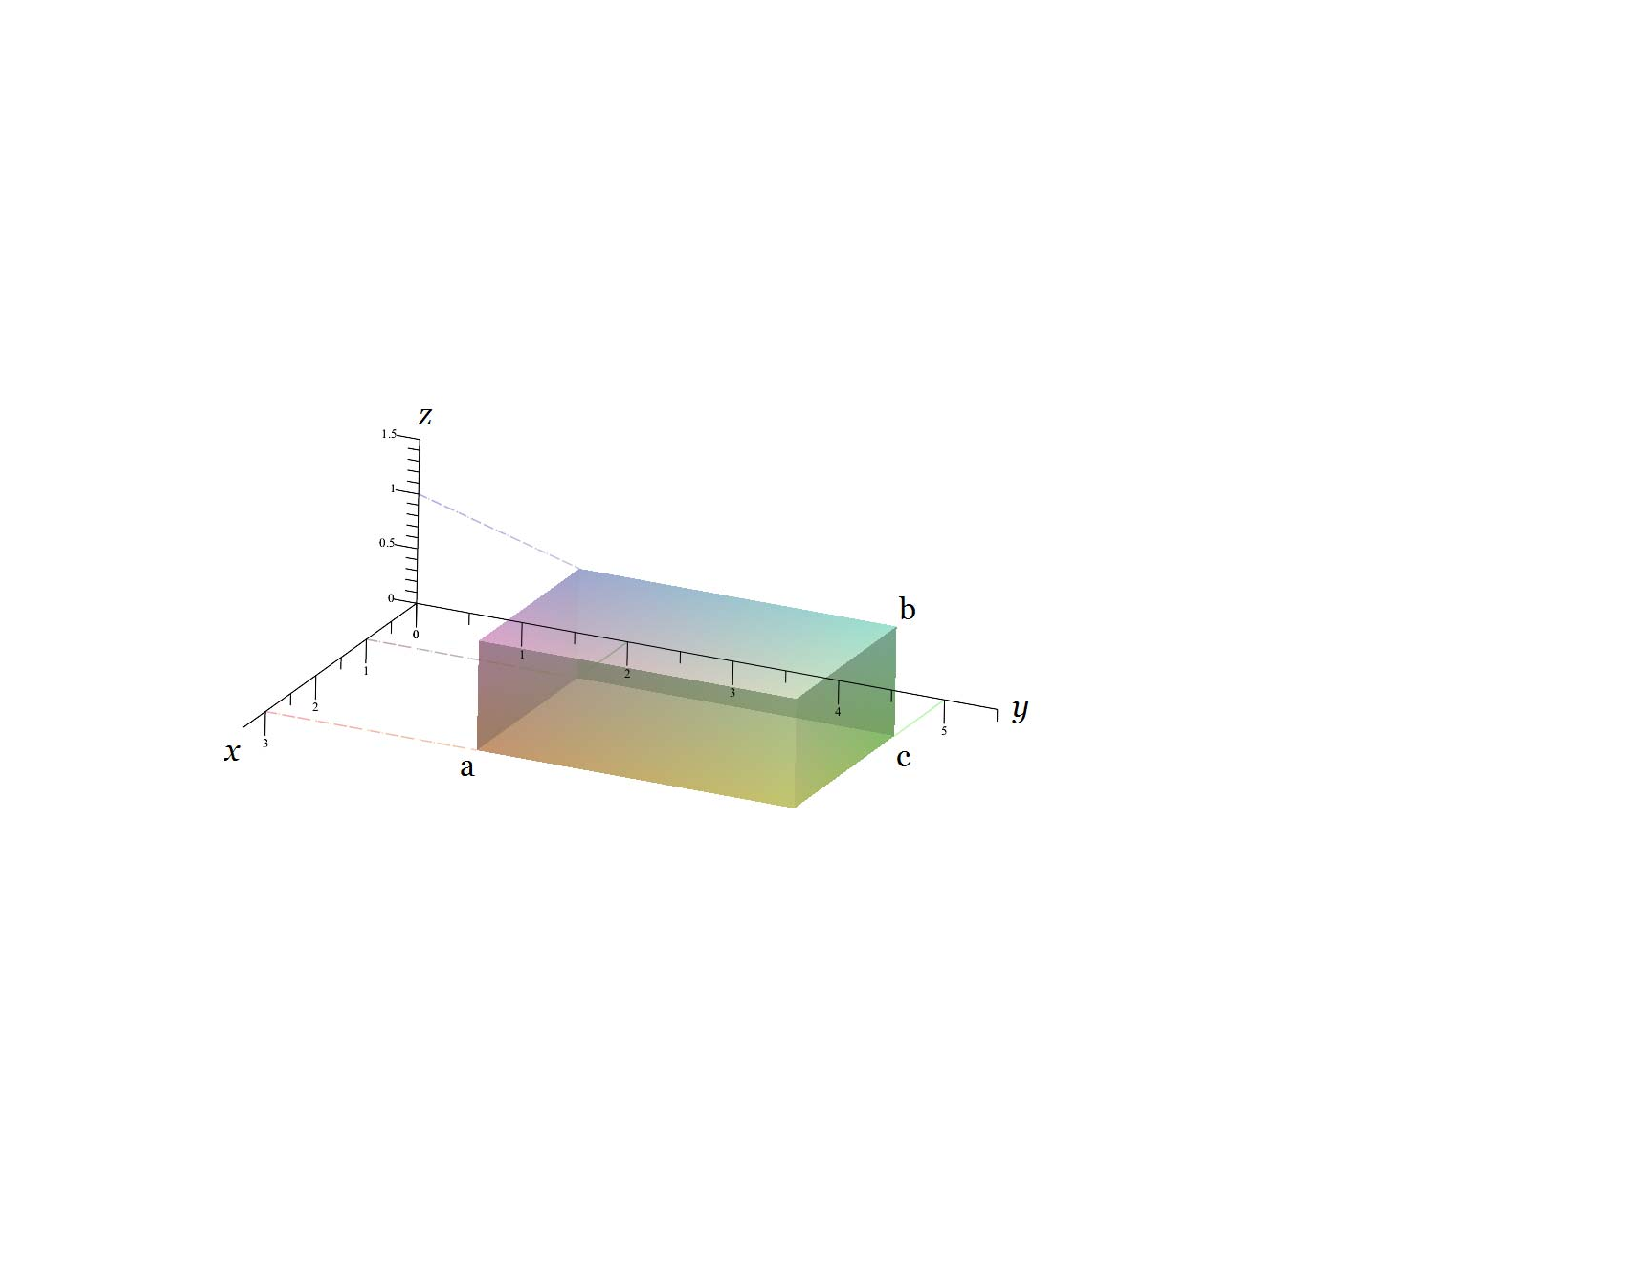
\includegraphics[scale=0.6]{box.pdf}
\end{center}
Use vectors to compute the angle between the diagonal which extends from vertex $a$ to vertex $b$ and the line segment which extends from vertex $a$ to vertex $c$. (Verify your answer with HW 11.1 \#3c.)

\includegraphics[scale=0.5]{start.pdf}
{{$\cos^{-1}\left(\frac{\sqrt{13}}{\sqrt{14}}\right)$}}
\includegraphics[scale=0.5]{end.pdf}


\item Consider the triangle, shown below,with vertices $A(1,-2,6)$, $B(3,0,-1)$, and $C(-2,1,0)$.
\begin{center}
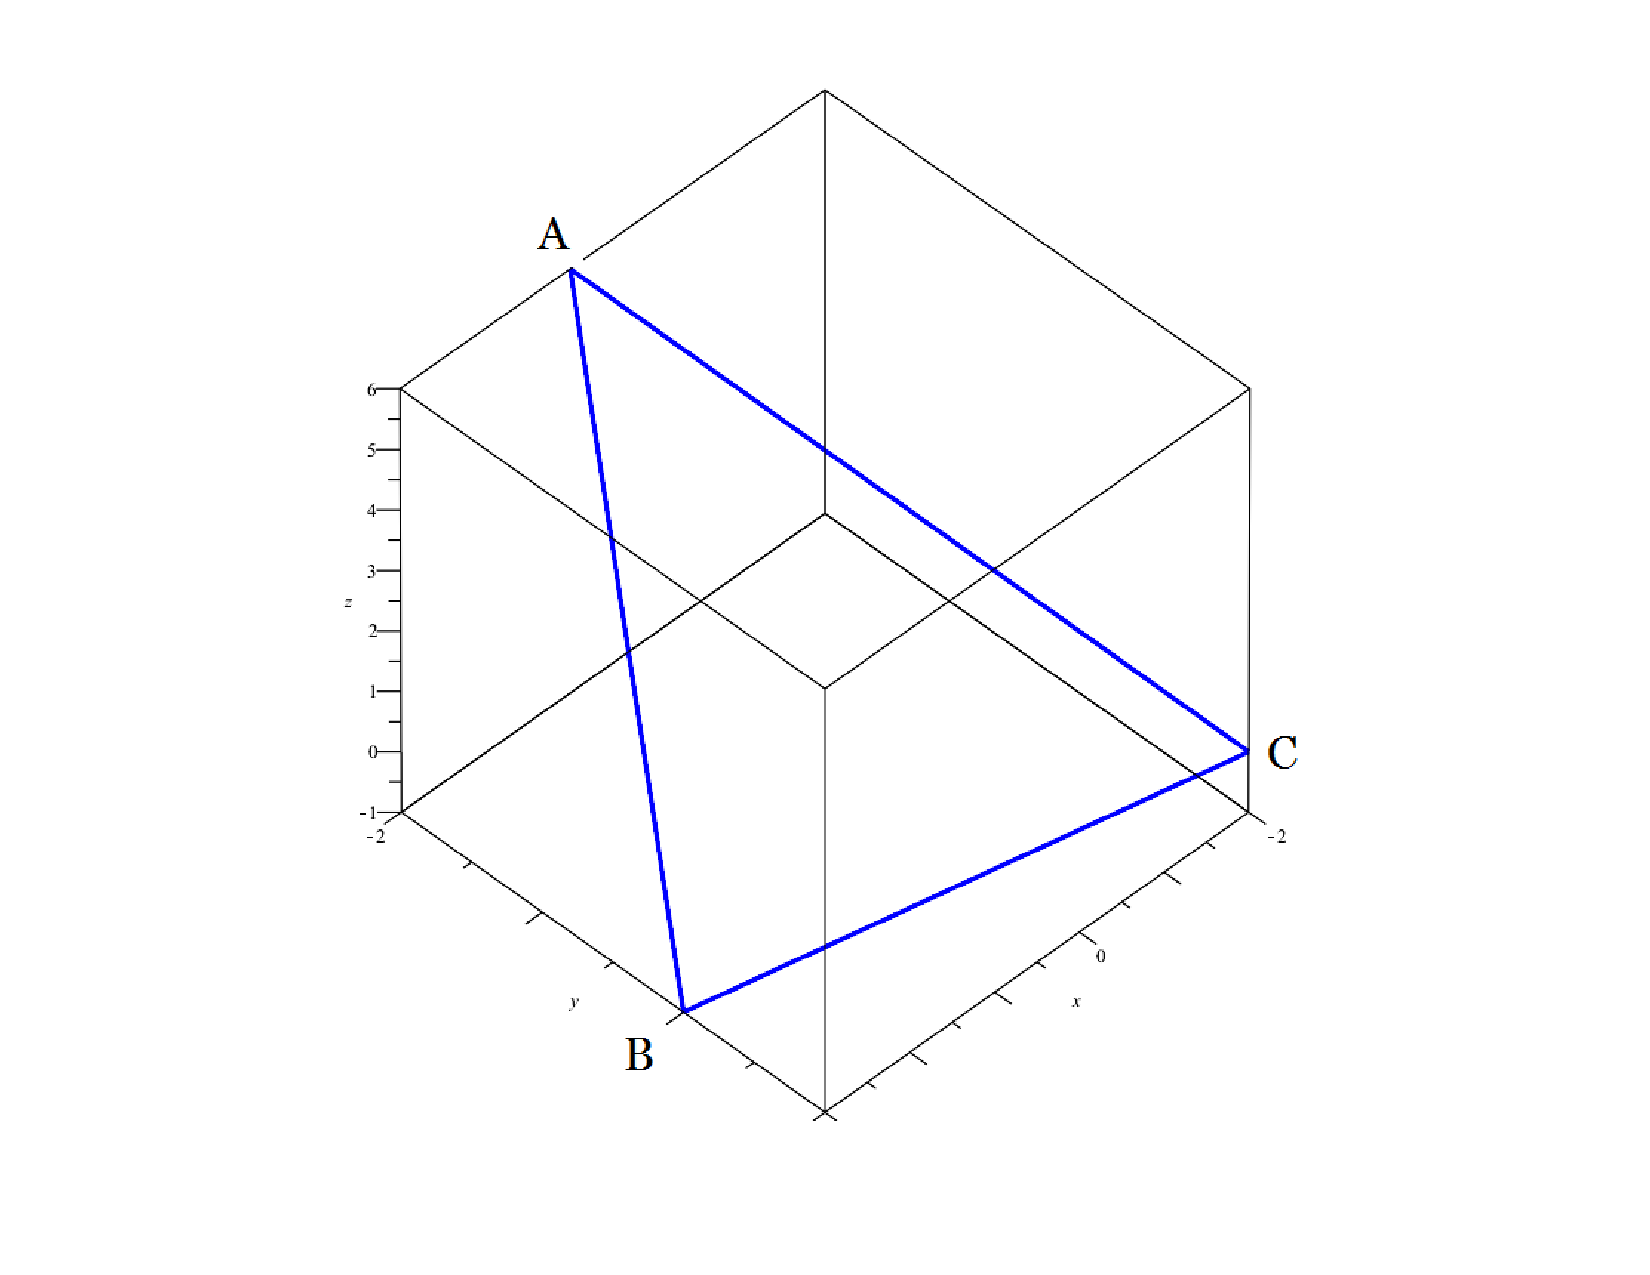
\includegraphics[scale=0.5]{triangle.pdf}
\end{center}
Compute all three angles of the triangle.

\newpage

\includegraphics[scale=0.5]{start.pdf}
{{{1\linewidth}{Angle $A$ has a measure of $\cos^{-1}\left(\frac{42}{\sqrt{57}\sqrt{54}}\right)$ radians.\\
Angle $B$ has a measure of $\cos^{-1}\left(\frac{15}{\sqrt{57}\sqrt{27}}\right)$ radians.\\
Angle $C$ has a measure of $\cos^{-1}\left(\frac{12}{\sqrt{54}\sqrt{27}}\right)$ radians.\\
(NOTE: Once you find any two of the angles, you can use the fact that the sum of all of the angles must be $\pi$ radians to compute the remaining angle.)
}}}
\includegraphics[scale=0.5]{end.pdf}
 

\item  Let $\overrightarrow{v}=\langle 1,2 \rangle$ and $\overrightarrow{b}=\langle -3,4 \rangle$.

\begin{enumerate}

\item Find the vector component of $\overrightarrow{v}$ along $\overrightarrow{b}$ and the vector component of $\overrightarrow{v}$ orthogonal to $\overrightarrow{b}$.  

\includegraphics[scale=0.5]{start.pdf}
{{{1\linewidth}{The vector component of $\overrightarrow{v}$ along $\overrightarrow{b}$ is $\text{Proj}_{\overrightarrow{b}}\overrightarrow{v}=\left\langle -\frac{3}{5},\frac{4}{5}\right\rangle$ and the vector component of $\overrightarrow{v}$ orthogonal to $\overrightarrow{b}$ is $\overrightarrow{v}-\text{Proj}_{\overrightarrow{b}}\overrightarrow{v}=\left\langle\frac{8}{5},\frac{6}{5}\right\rangle$.}}}
\includegraphics[scale=0.5]{end.pdf}


\item Sketch $\overrightarrow{v}$, $\overrightarrow{b}$, and the vector components that you found in part (a).

\includegraphics[scale=0.5]{start.pdf}
{{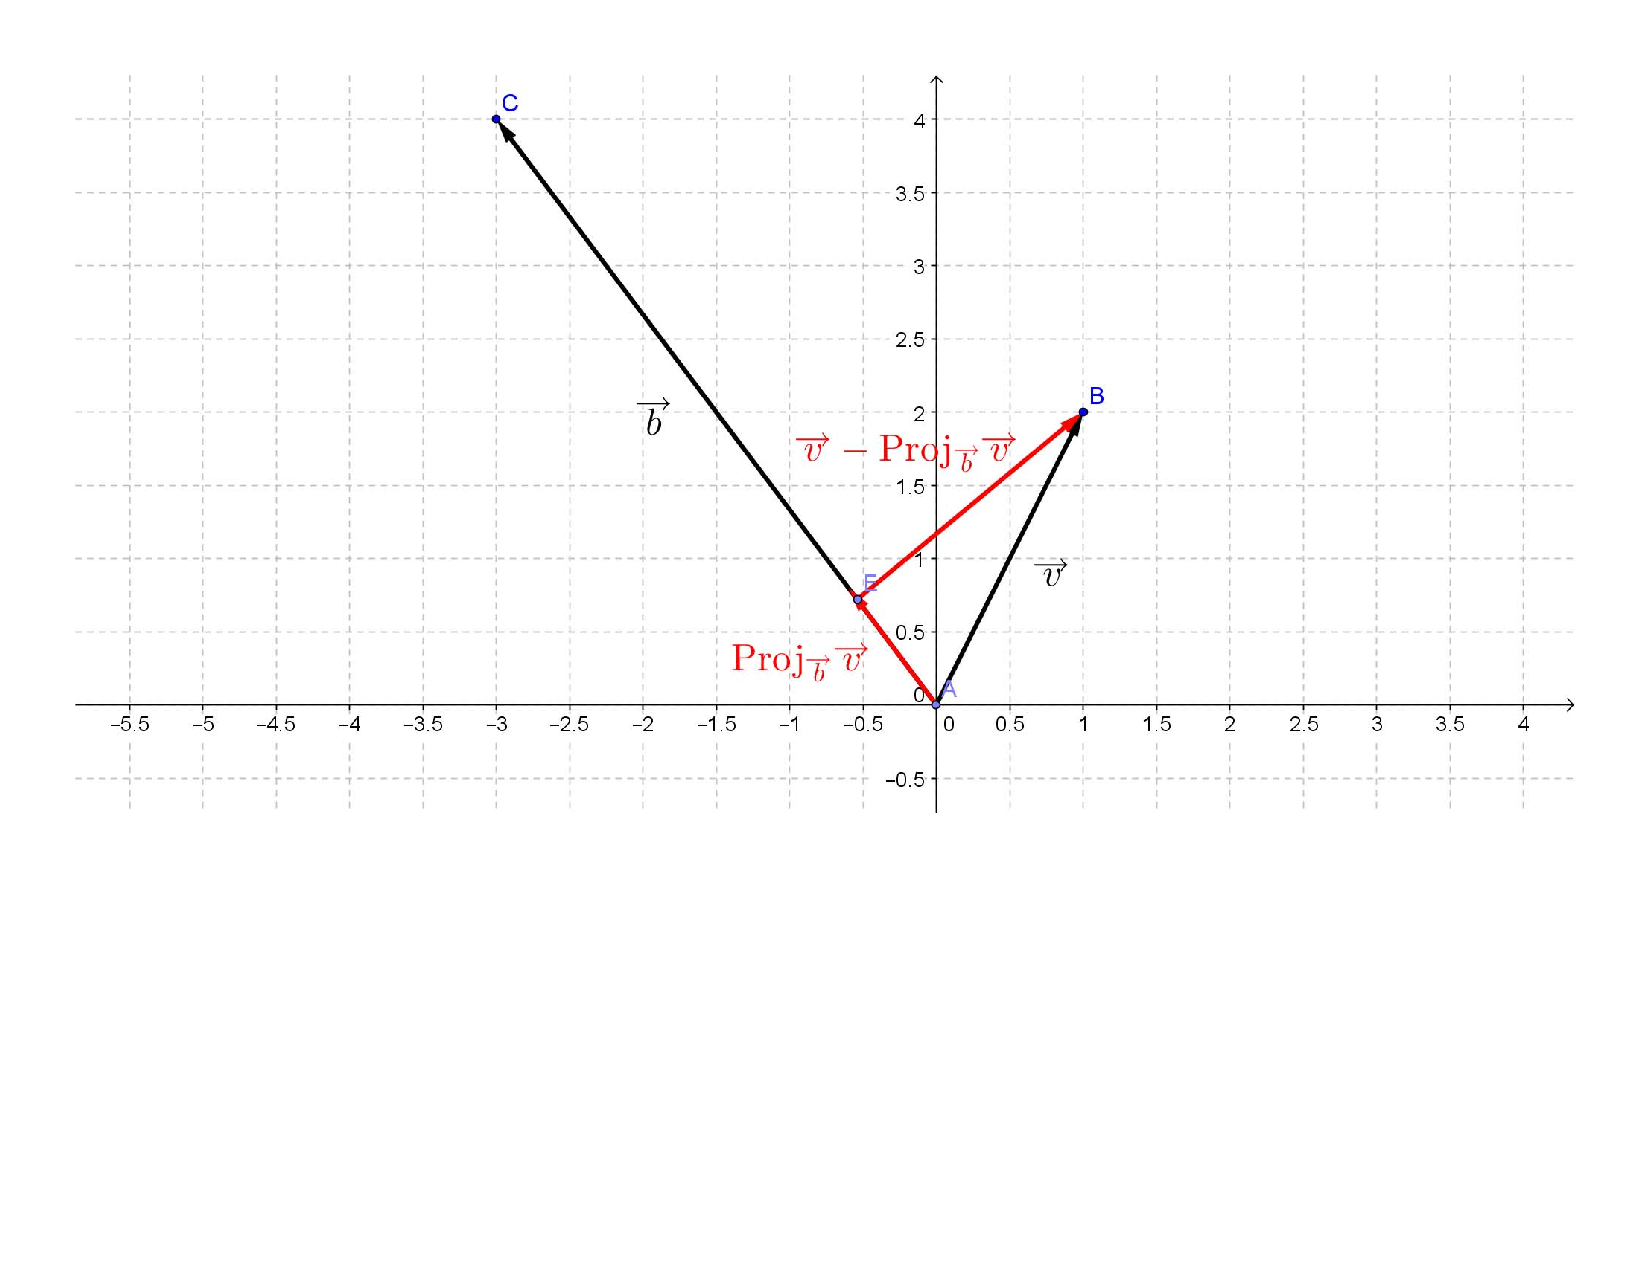
\includegraphics[scale=0.4]{projection.pdf}}}
\includegraphics[scale=0.5]{end.pdf}


\end{enumerate}

\item Express ${\bf v}={\bf i}+2{\bf j}+3{\bf k}$ as the sum of a vector parallel to ${\bf b}=-2{\bf i}+4{\bf j}-{\bf k}$ and a vector perpendicular to ${\bf b}$

\includegraphics[scale=0.5]{start.pdf}
{{${\bf v}=\left\langle-\frac{2}{7},\frac{4}{7},-\frac{1}{7}\right\rangle+\left\langle \frac{9}{7},\frac{10}{7},\frac{22}{7}\right\rangle$}}
\includegraphics[scale=0.5]{end.pdf}


\item Suppose that ${\bf u} \neq {\bf 0}$ and ${\bf v} \neq {\bf 0}$.  Under what condition will $\|{\bf u}+{\bf v}\|=\|{\bf u}-{\bf v}\|$?  Explain.

\includegraphics[scale=0.5]{start.pdf}
{{The result follows if ${\bf u}$ is orthogonal to ${\bf v}$.}}
\includegraphics[scale=0.5]{end.pdf}


\item The following questions deal with finding the distance from a point to a line:

\begin{enumerate}

\item Given three points $A$, $B$, and $P$ in 2-space or 3-space as shown in the picture below, describe two different ways that you could use the dot product to calculate the distance, $d$, between the point $P$ and the line which contains $A$ and $B$.

\begin{center}
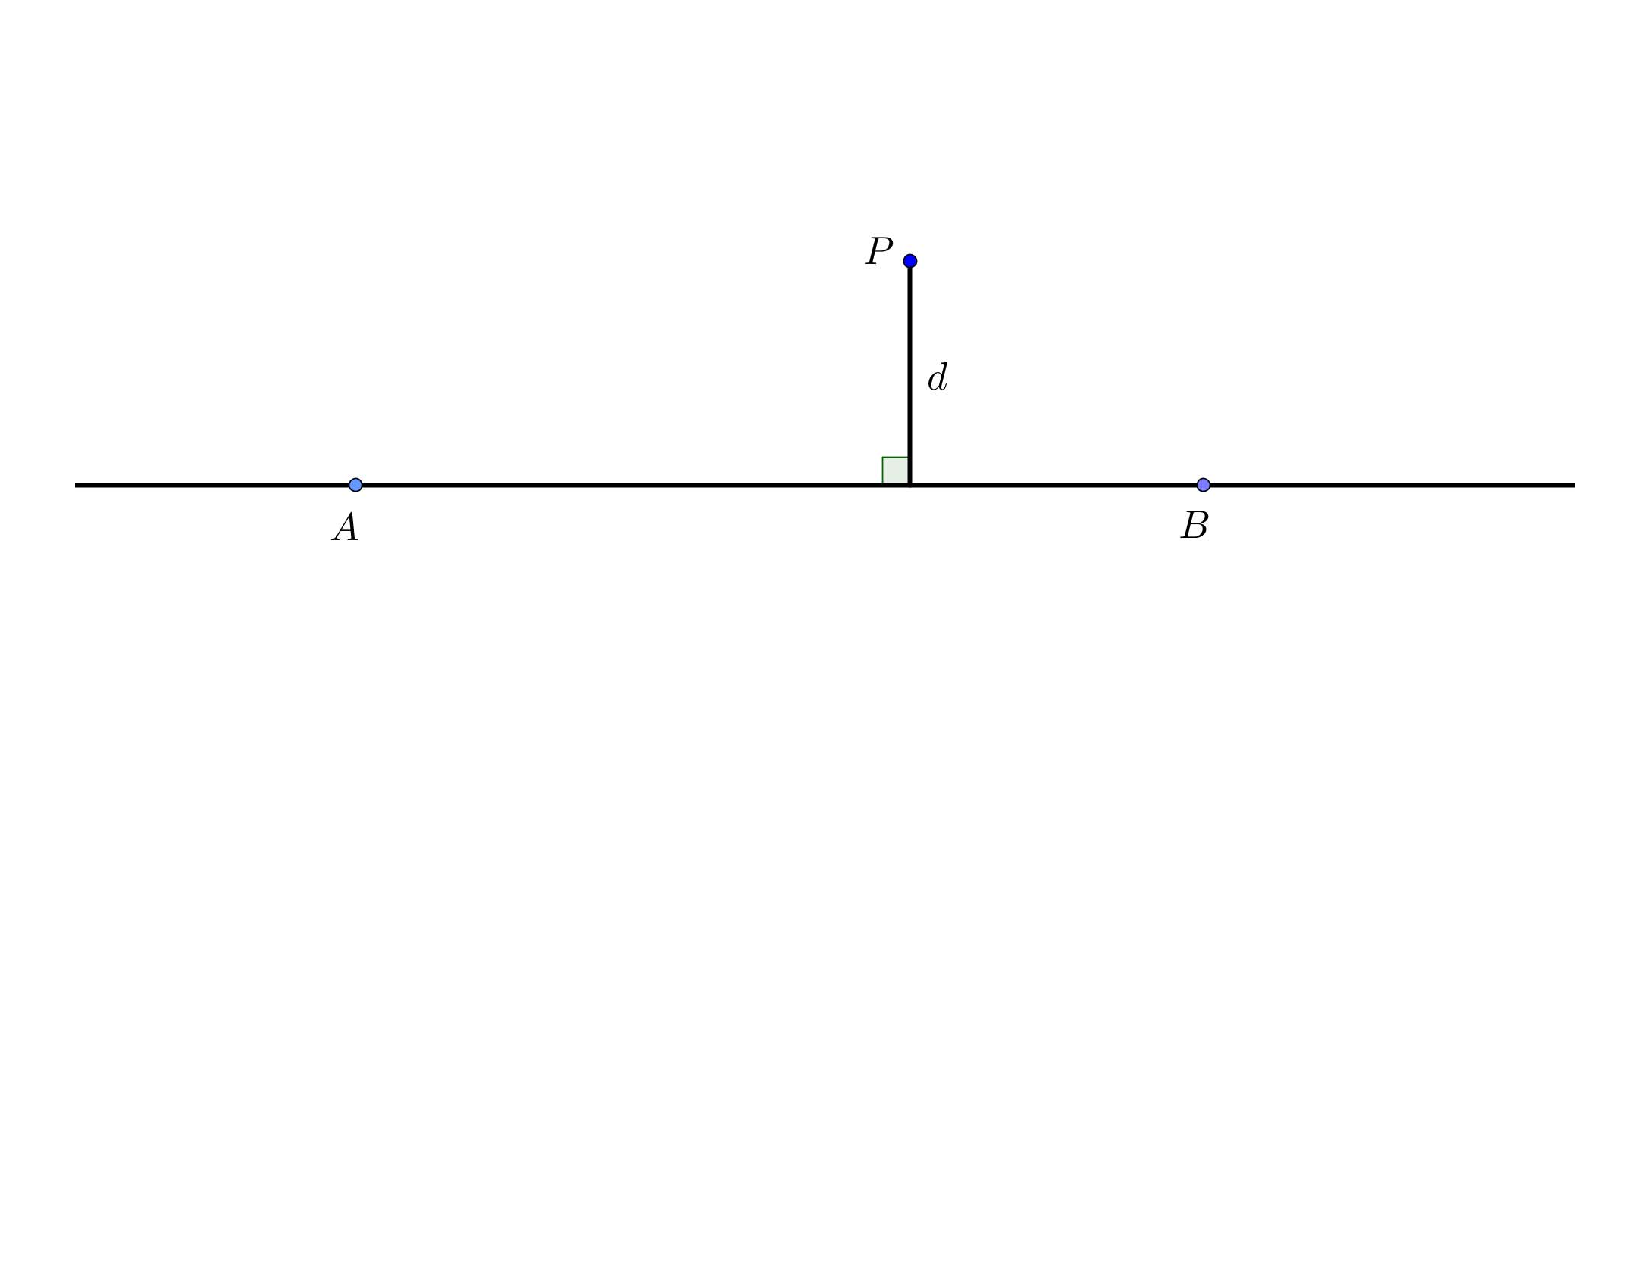
\includegraphics[scale=0.5]{length.pdf}
\end{center}

\includegraphics[scale=0.5]{start.pdf}
{{{1\linewidth}{\underline{OPTION 1:}\\
One can compute $\left\|\overrightarrow{AP}\right\|$ and $\left\|\text{Proj}_{\overrightarrow{AB}}\overrightarrow{AP}\right\|$.  Then, use Pythagorean Theorem to calculate $d$.\\
\\
\underline{OPTION 2:}\\
One can compute $\text{Proj}_{\overrightarrow{AB}}\overrightarrow{AP}$.  Then, $d=\left\|\overrightarrow{AP}-\text{Proj}_{\overrightarrow{AB}}\overrightarrow{AP}\right\|$.}}}
\includegraphics[scale=0.5]{end.pdf}


\item Use one of your methods from part (a) to compute the distance from the point $P(5,3,0)$ to the line containing $A(1,0,1)$ and $B(2,3,1)$.

\includegraphics[scale=0.5]{start.pdf}
{{$d=\sqrt{\frac{91}{10}}$}}
\includegraphics[scale=0.5]{end.pdf}


\end{enumerate}

\item Consider the triangle shown below which is formed by vectors ${\bf v}$ and ${\bf w}$.

\begin{center}
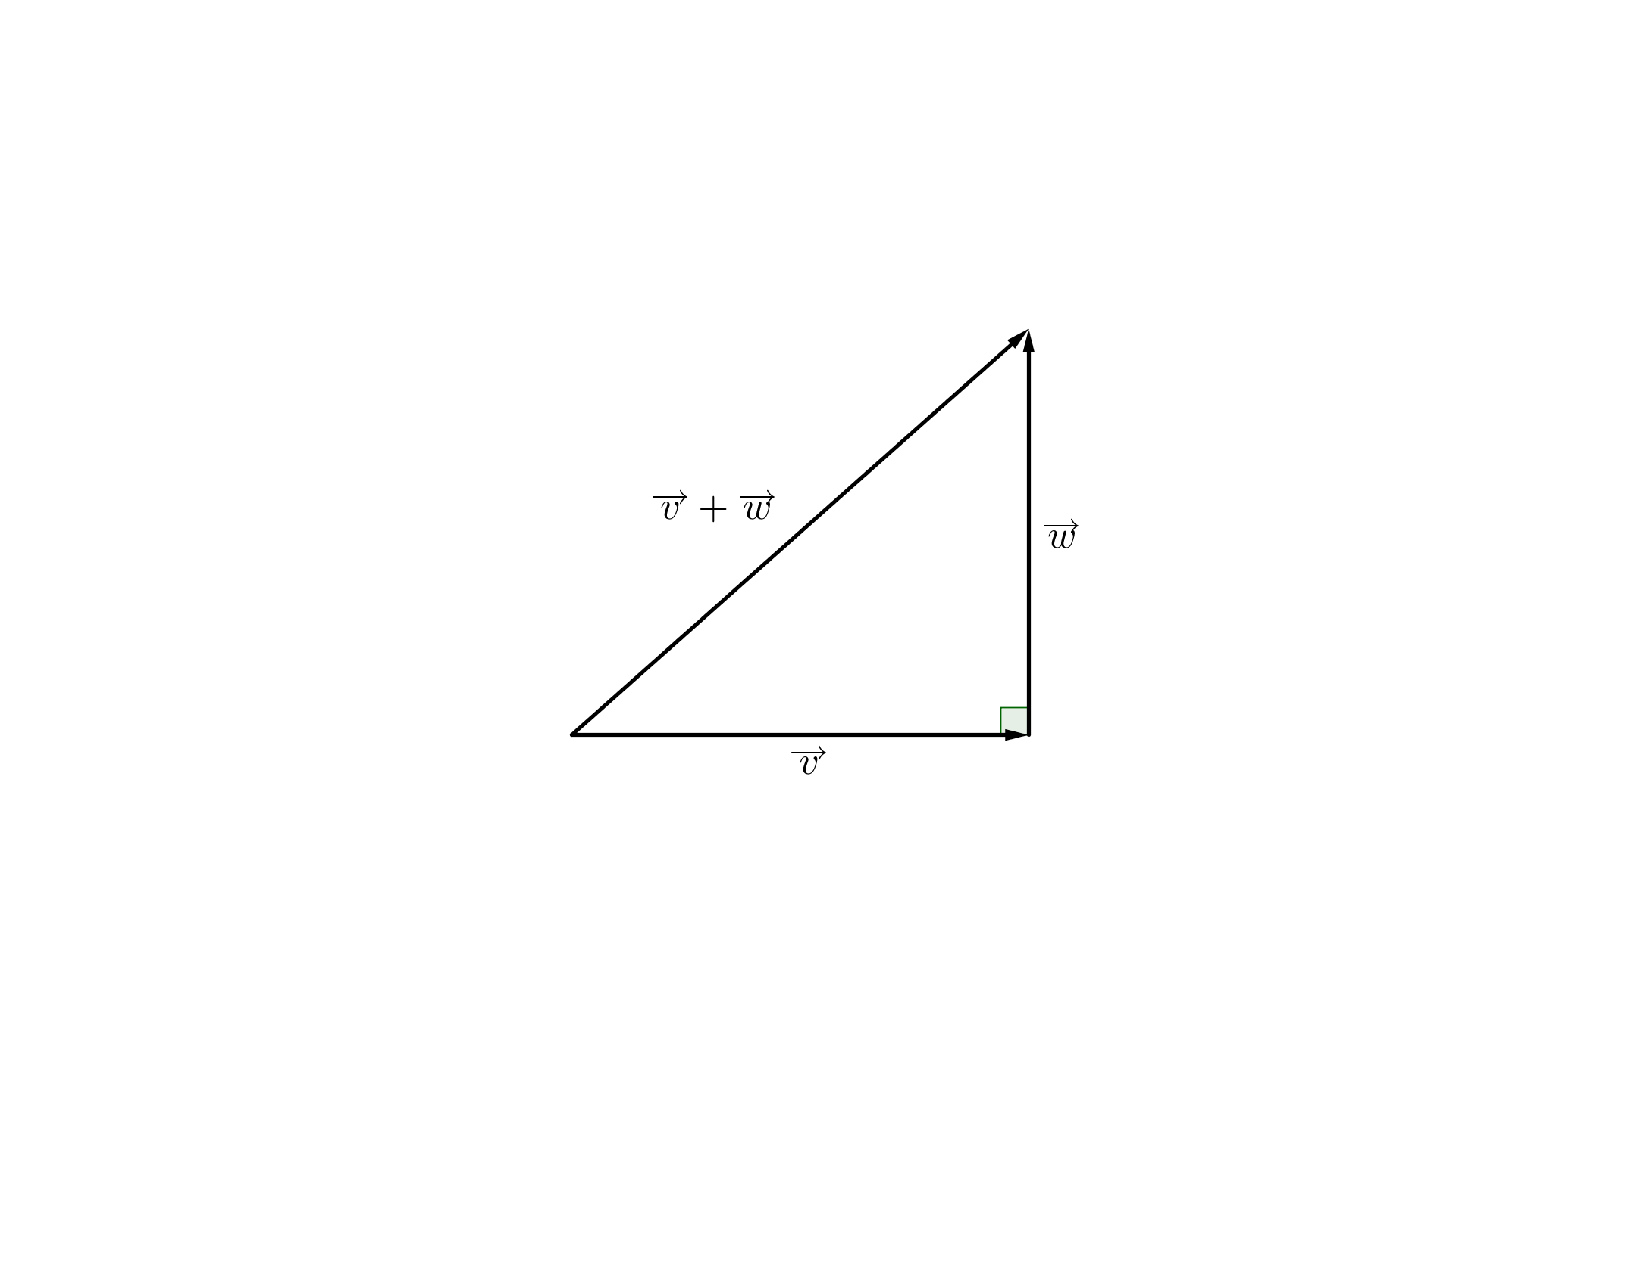
\includegraphics[scale=0.5]{Pythag.pdf}
\end{center}

Prove Pythagorean's Theorem $\|{\bf v}+{\bf w}\|^2=\|{\bf v}\|^2+\|{\bf w}\|^2$.  (Hint: Use properties of the dot product to expand $\|{\bf v}+{\bf w}\|^2$.)

\includegraphics[scale=0.5]{start.pdf}
{{{1\linewidth}{We expand $\|{\bf v}+{\bf w}\|^2$ using properties of the dot product:
\begin{align*}
\|{\bf v}+{\bf w}\|^2&=({\bf v}+{\bf w})\cdot({\bf v}+{\bf w})\\
&={\bf v}\cdot{\bf v}+{\bf v}\cdot{\bf w}+{\bf w}\cdot{\bf v}+{\bf w}\cdot{\bf w}\\
&=\|{\bf v}\|^2+2({\bf v}\cdot {\bf w})+\|{\bf w}\|^2 \text{ (since } {\bf v}\cdot {\bf w}={\bf w}\cdot {\bf v})\\
&=\|{\bf v}\|^2+\|{\bf w}\|^2 \text{ (since }{\bf v}\perp{\bf w}\Leftrightarrow {\bf v}\cdot{\bf w}=0)
\end{align*}
Thus, $\|{\bf v}+{\bf w}\|^2=\|{\bf v}\|^2+\|{\bf w}\|^2$, as promised.
}}}
\includegraphics[scale=0.5]{end.pdf}


\item Let $A$ and $B$ be endpoints of a diameter of a circle with a radius of $r$ .  And, suppose that $C$ is any other point on the circle, as shown below. 
\begin{center}
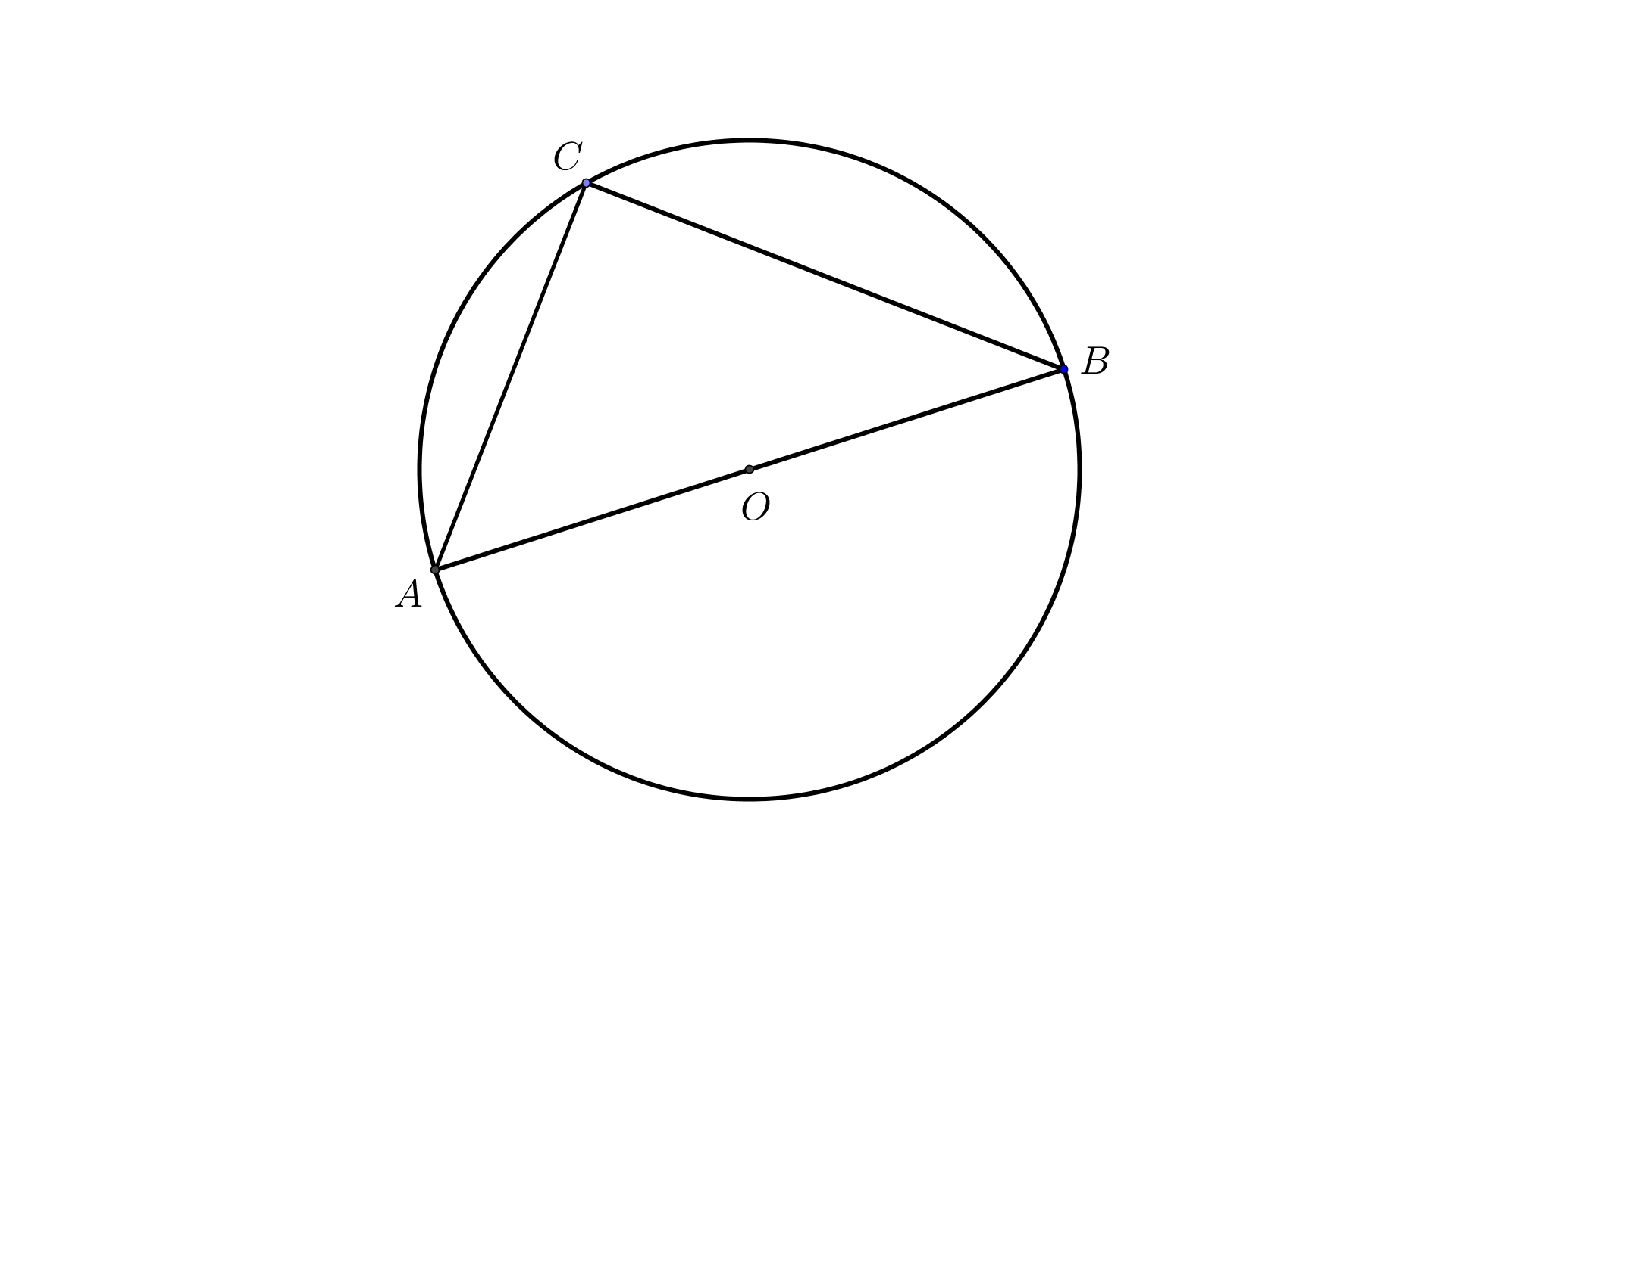
\includegraphics[scale=0.5]{circle.pdf}
\end{center}
 Prove that triangle $ABC$ is a right triangle.  (Hint: Express each of $\overrightarrow{CA}$ and $\overrightarrow{CB}$ as the combination of $\overrightarrow{CO}$ and some other vector.)

\includegraphics[scale=0.5]{start.pdf}
{{{1\linewidth}{Notice that ${\bf CA}={\bf CO}+{\bf OA}$ and ${\bf CB}={\bf CO}+{\bf OB}$.  But, ${\bf OB}=-{\bf OA}$.  Thus, ${\bf CB}={\bf CO}-{\bf OA}$.  We will show that ${\bf CA} \perp {\bf CB}$ by showing that ${\bf CA} \cdot {\bf CB}=0$.
\begin{align*}
{\bf CA}\cdot {\bf CB}&=\left({\bf CO}+{\bf OA}\right) \cdot \left({\bf CO}-{\bf OA}\right)\\
&= {\bf CO}\cdot{\bf CO}-{\bf CO}\cdot {\bf OA}+{\bf OA}\cdot{\bf CO}-{\bf OA}\cdot{\bf OA}\\
&=\|{\bf CO}\|^2-\|{\bf OA}\|^2\\
&=r^2-r^2\\
&=0
\end{align*}
So, ${\bf CA}\perp{\bf CB}$ and the triangle is a right triangle.
}}}
\includegraphics[scale=0.5]{end.pdf}


\item Let $\overrightarrow{v}$ and $\overrightarrow{w}$ be vectors, either both in $\mathbb{R}^2$ or in $\mathbb{R}^3$.  Prove the Cauchy-Schwarz Inequality: $|\overrightarrow{v}\cdot \overrightarrow{w}|\leq \|\overrightarrow{v}\|\|\overrightarrow{w}\|$.

\includegraphics[scale=0.5]{start.pdf}
{{{1\linewidth}{
Suppose that $\theta$ is the angle between $\overrightarrow{v}$ and $\overrightarrow{w}$.  Then:
\begin{align*}
|\overrightarrow{v}\cdot\overrightarrow{w}|&=\left|\|\overrightarrow{v}\|\|\overrightarrow{w}\|\cos{\theta}\right|\\
&=\left(\|\overrightarrow{v}\|\right)\left(\|\overrightarrow{w}\|\right)\left(|\cos{\theta}|\right)\\
&\leq\left(\|\overrightarrow{v}\|\right)\left(\|\overrightarrow{w}\|\right)(1)\\
&=\|\overrightarrow{v}\| \|\overrightarrow{w}\|
\end{align*}
Thus, $|\overrightarrow{v}\cdot \overrightarrow{w}|\leq \|\overrightarrow{v}\|\|\overrightarrow{w}\|$, as promised.
}}}
\includegraphics[scale=0.5]{end.pdf}


\item Let $\overrightarrow{v}=\langle 1,2,3 \rangle$.

\begin{enumerate}

\item Compute the direction cosines of $\overrightarrow{v}$.

\includegraphics[scale=0.5]{start.pdf}
{{{1\linewidth}{Let $\alpha$, $\beta$, and $\gamma$ be the angles between $\overrightarrow{v}$ and ${\bf i}$, ${\bf j}$, and ${\bf k}$, respectively.  Then:\\ $\cos{\alpha}=\frac{1}{\sqrt{14}}$, $\cos{\beta}=\frac{2}{\sqrt{14}}$, and $\cos{\gamma}=\frac{3}{\sqrt{14}}$}}}
\includegraphics[scale=0.5]{end.pdf}


\item Verify that $\cos^2\alpha+\cos^2\beta+\cos^2\gamma=1$, where $\alpha$, $\beta$, and $\gamma$ be the angles between $\overrightarrow{v}$ and ${\bf i}$, ${\bf j}$, and ${\bf k}$, respectively.

\includegraphics[scale=0.5]{start.pdf}
{{{1\linewidth}{Using the information from part (a), we obtain:
\begin{align*}
\cos^2\alpha+\cos^2\beta+\cos^2\gamma&=\left(\frac{1}{\sqrt{14}}\right)^2+\left(\frac{2}{\sqrt{14}}\right)^2+\left(\frac{3}{\sqrt{14}}\right)^2\\
&=\frac{1}{14}+\frac{4}{14}+\frac{9}{14}\\
&=1
\end{align*}
}}}
\includegraphics[scale=0.5]{end.pdf}


\end{enumerate}

\end{enumerate}

\end{document}